\subsubsection{Herde}\label{sec:Reiseherde}

\begin{figure*}[tb]
\centering
\begin{subfigure}[t]{\columnwidth}
 \centering
 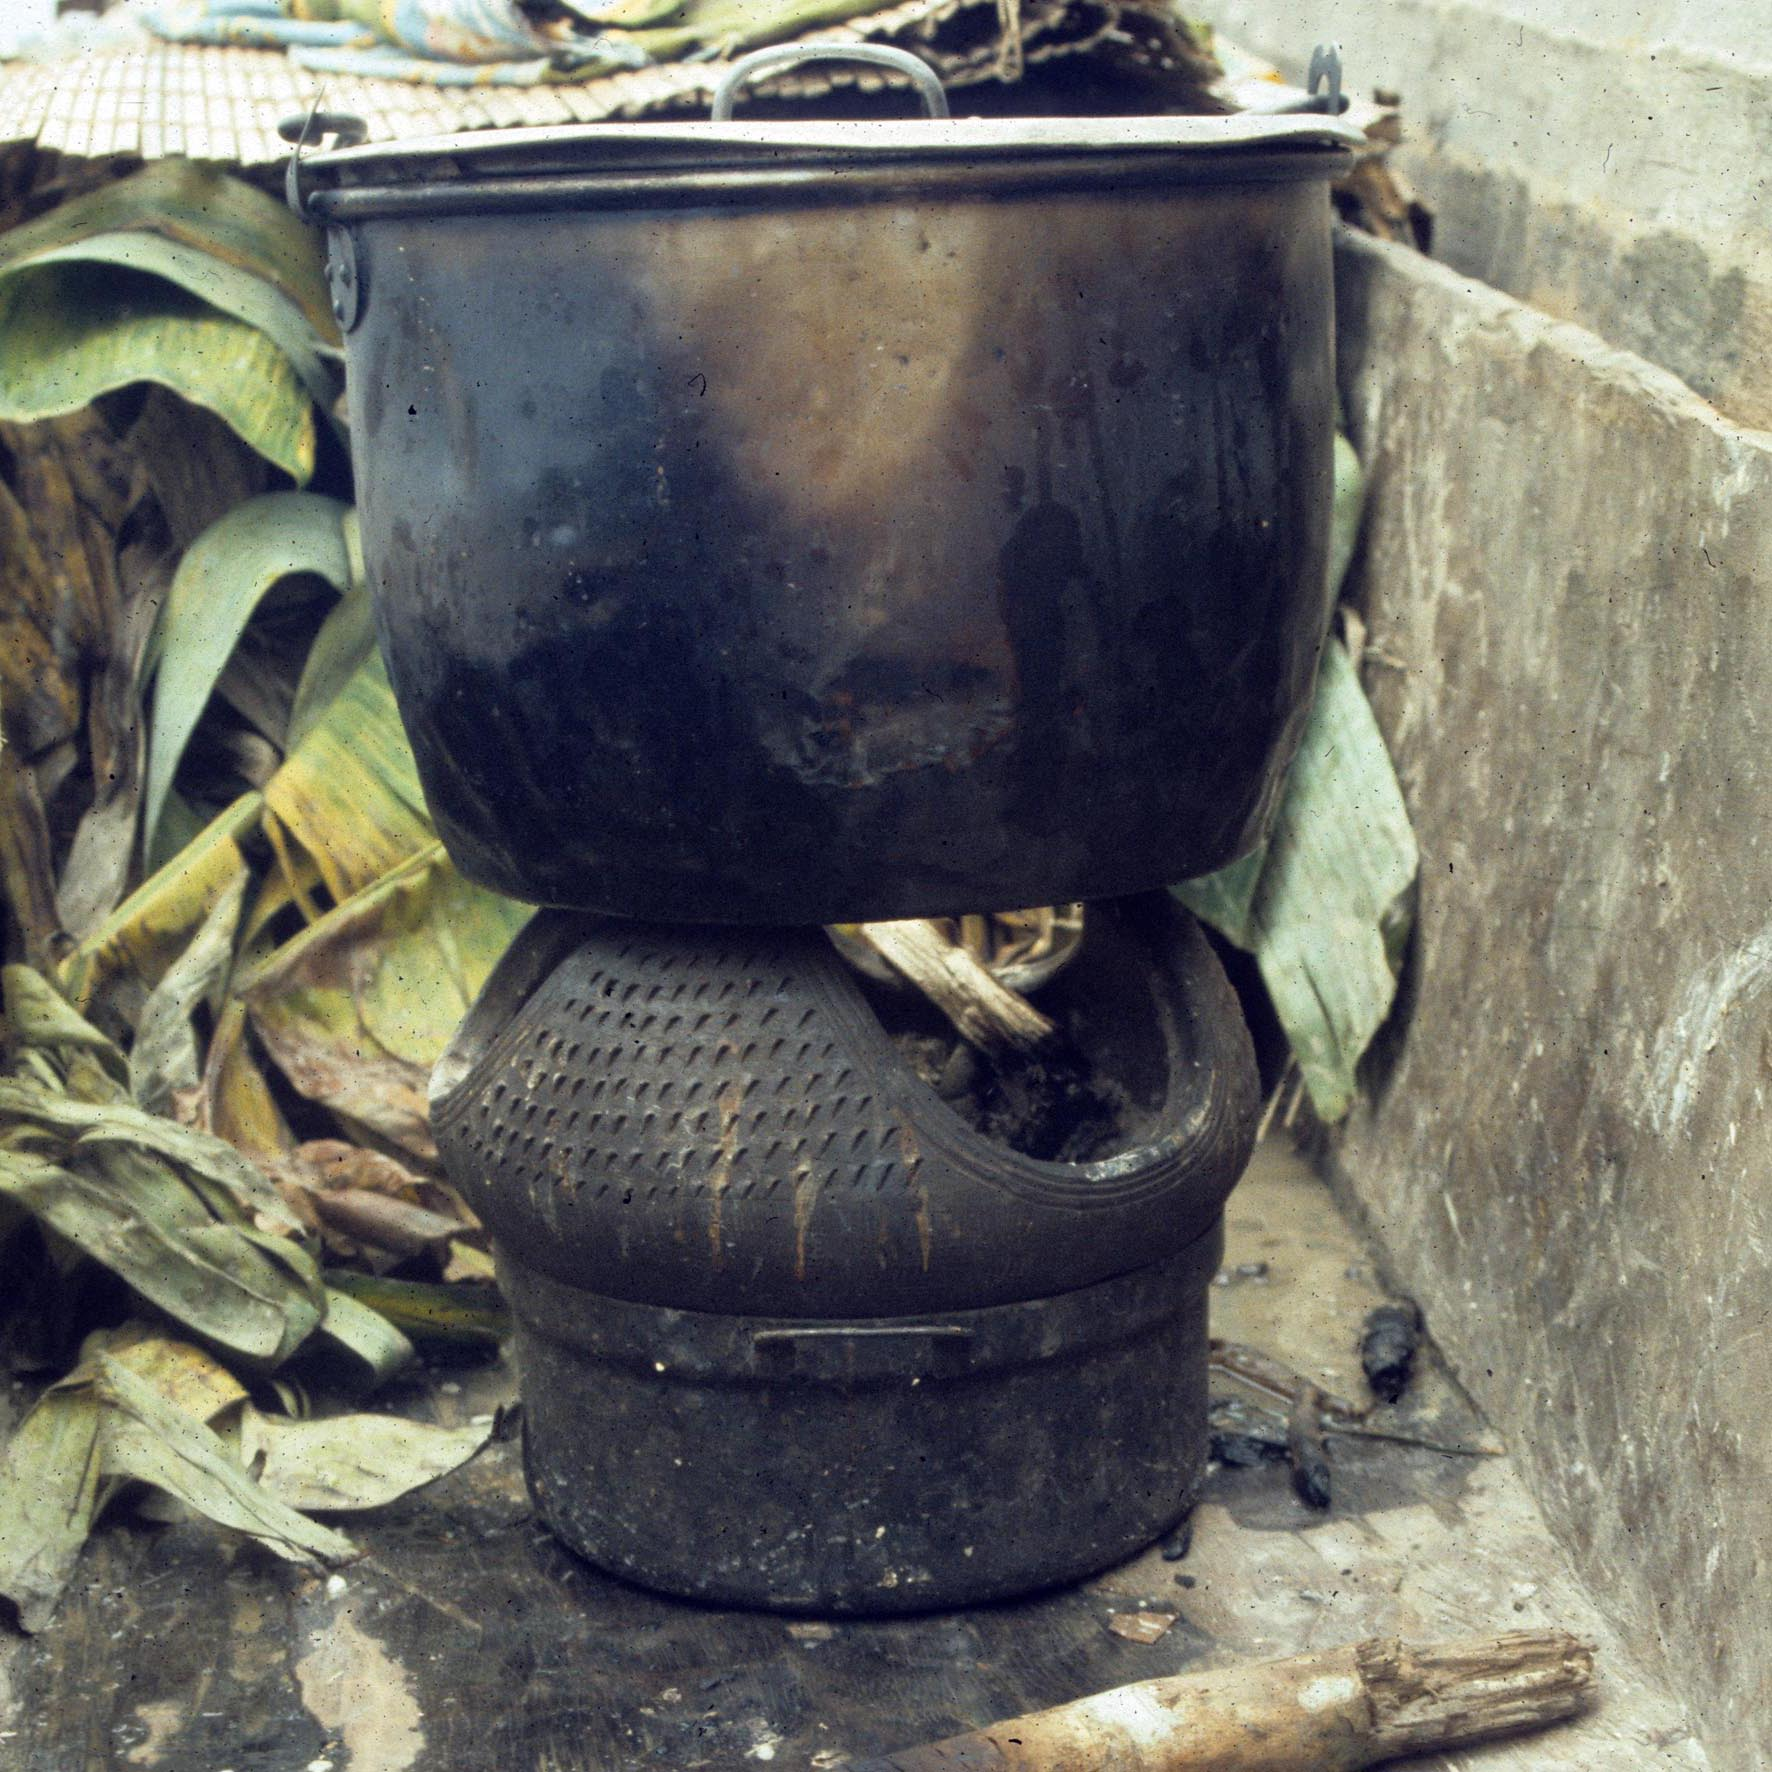
\includegraphics[width=\textwidth]{fig/UBA85-100_Ubangi-km100_12-08-85.jpg}
 \caption{\mbox{Ubangi} Flusskilometer 100 (UBA 85/100): Situationsfoto eines Einbaums mit einem als \enquote*{\textit{ik$\varepsilon$ng$\varepsilon$}} bezeichneten Reiseherd mit drei Hörnern. Der Herd selbst steht auf einem Metallgefäß und auf ihm befindet sich eine metallenes Kochgefäßes (Foto: M. K. H. Eggert, 1985).}
 \label{fig:Reiseherd_A}
\end{subfigure}\hfill
\begin{subfigure}[t]{\columnwidth}	
 \centering
 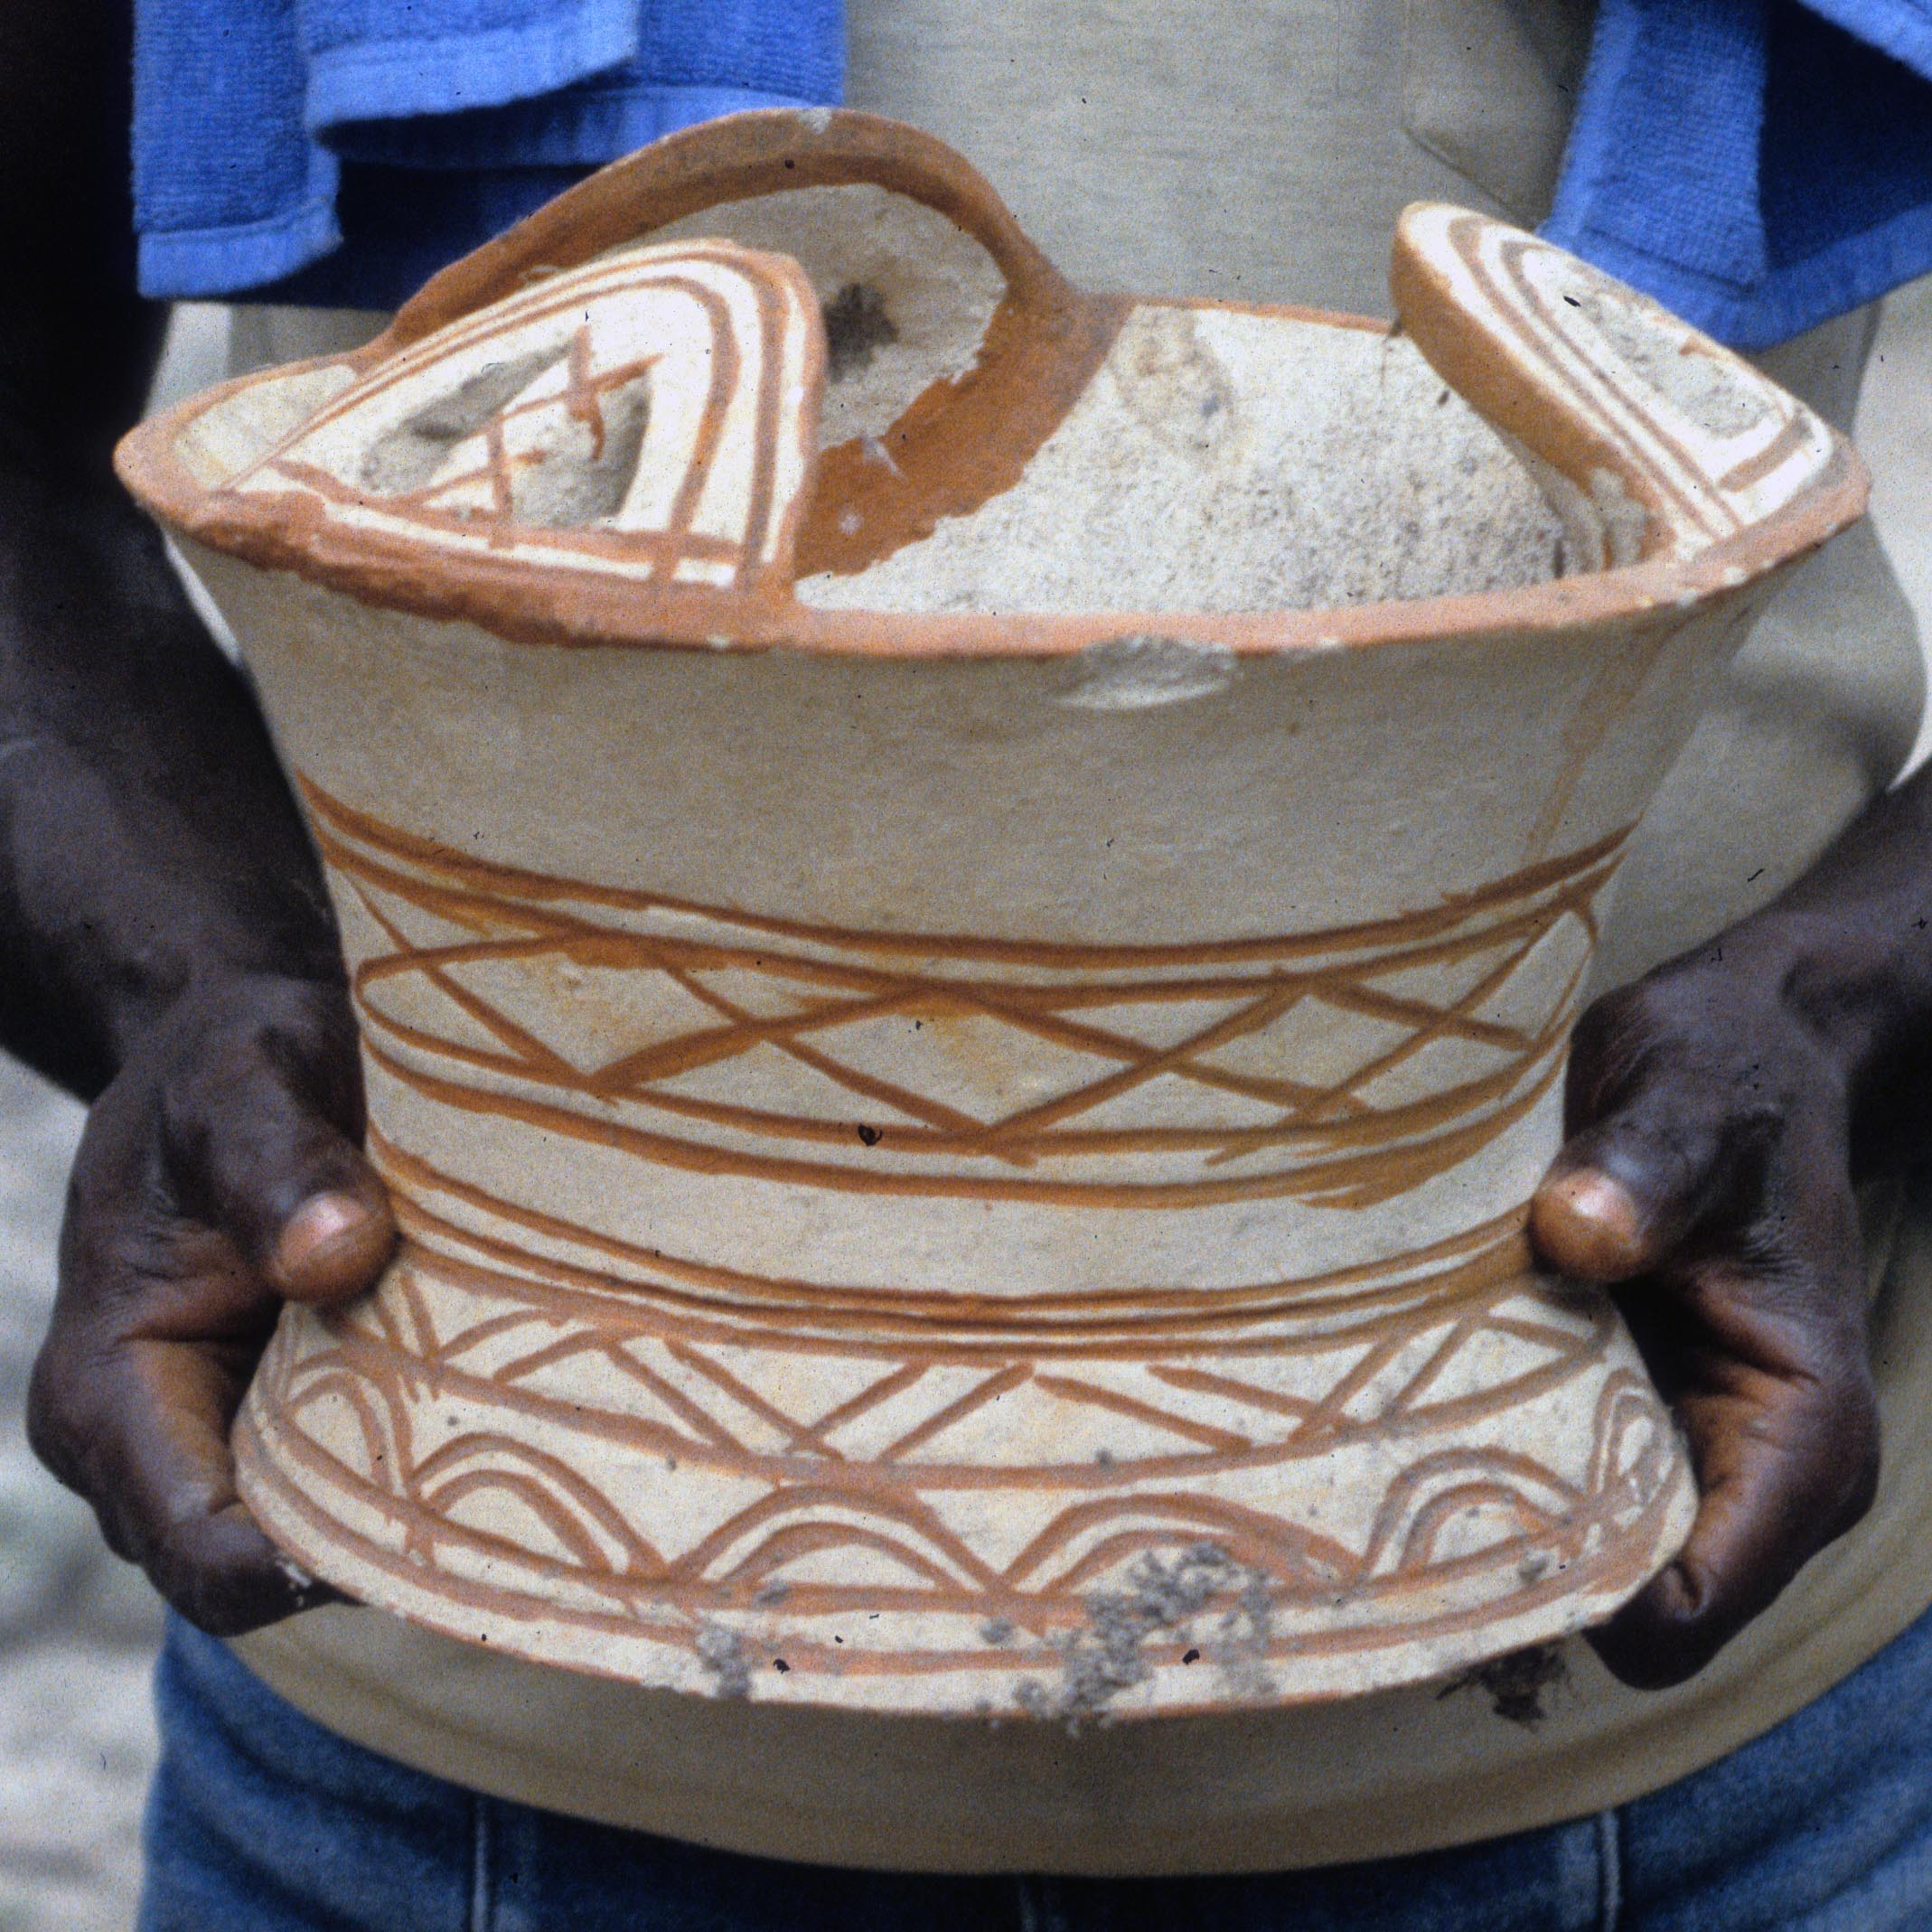
\includegraphics[width=\textwidth]{fig/BBS87_Herdgef_E87-04-4.jpg}
 \caption{Bobusa (Fpl.~239): Reiseherd mit roter Bemalung (Foto: M. K. H. Eggert, 1987).}
 \label{fig:Reiseherd_B}
\end{subfigure}
 \caption{Reiseherd: Während der Feldaufenthalte beobachtete Reiseherde mit drei \enquote{Hörnern}.}
 \label{fig:Reiseherd}
\end{figure*}

Eine weitere Kategorie innerhalb des keramischen Fundmaterials bilden die sogenannten \enquote{Reiseherde}. Alle im Arbeitsgebiet beobachteten Vertreter dieses funktionalen Gefäßtyps folgen einem formalen Grundprinzip: es handelt sich um offene Gefäße mit Standringboden (B13), an deren Oberseite regelhaft drei \textit{Hörner} beziehungsweise Vorsätze herausgearbeitet oder angebracht sind (Abb.~\ref{fig:Reiseherd}).\footnote{Die Proportionen der Reiseherde wurden entsprechend der Messtrecken für die Gefäßkeramik aufgenommen (Abb.~\ref{fig:GefAbmessungen_Schema}). Die Öffnungsweite am Rand der Reiseherde liegt zwischen 18 und 40\,cm und die Höhe bei etwa 16--18\,cm. Die Reiseherde weisen allesamt Böden mit einem Standring auf (Bodenform B13; Taf.~39.1--2, 74.1, 79.3).} Auf diese Vorsätze wird das Kochgefäß aufgestellt, während der Herd das Brenngut aufnimmt (Abb.~\ref{fig:Reiseherd_A}). In zwei Fällen war zu beobachten, dass die Vorsätze als separat ausgeformte Elemente über einen an der Verbindungsstelle herausgearbeiteten, dreieckigen Keil am Gefäß befestigt wurden (Taf.~79.2).\footnote{Am \textit{Horn} beziehungsweise dem Vorsatz wurde ein dreieckiger Keil herausgearbeitet, der in eine entsprechende Aussparung am Gefäßkörper des Reiseherdes eingreift. Dies belegt die separate Fertigung der Einzelteile. Da sich Brüche genau in diesem Bereich ergaben, kann davon ausgegangen werden, dass die Anbringung der Vorsätze an den Gefäßkörper im lederharten Zustand erfolgte.} Im letzteren Fall lassen sich auch feine vertikale Riefen im Bereich der Verbindungsstelle erkennen, die möglicherweise ausgearbeitet wurde um eine bessere Verbindung zu erzeugen.

Das Fundinventar umfasst 35 Reiseherde oder Fragmente von Reiseherden aus 14 verschiedenen Fundplätzen (Taf.~38.16, 39.1--2, 56.12, 74.1, 79.2--3). Das Gros der Reiseherde stammt von Fundstellen entlang des unteren und mittleren \mbox{Sangha} (68,5\,\%). Von Fundstellen entlang des Unterlaufs des \mbox{Likwala}-\mbox{aux}-\mbox{Herbes} liegen sieben Objekte vor (20\,\%), während lediglich an jeweils zwei Fundstellen entlang des unteren \mbox{Ubangi} sowie des befahrenen Abschnitts des Kongo Reiseherde erfasst wurden. Bei Grabungen wurden lediglich zwei Fragmente entsprechender Herde entdeckt, beide stammen aus der rezenten Grube PIK~87/2 (Kat.-Nr.~9) in Pikunda (Fpl.~255). Alle übrigen Stücke stammen aus Oberflächensurveys. Die regionale Verbreitung der im Fundgut enthaltenen Reiseherde zeichnet diese als ein Phänomen des südlichen Randes des Arbeitsgebietes aus. Nördlich von Itanga (Fpl.~192) am \mbox{Ubangi} sowie Itandi (Fpl.~256) am \mbox{Sangha} liegen keine Belege für die Nutzung von Reiseherden vor.

Auffällig ist, dass fast alle untersuchten Fragmente Schamott-Magerung und somit einen Scherben des \textit{Fabric} 9 aufweisen (88\,\%). Die einzigen Stücke, die jedoch lediglich potenziell den hier genannten mobilen Herden zugerechnet werden können und keine Schamott-Magerung aufwiesen, sind je ein Bodenframgent mit Standring aus Ilebo (Fpl.~287), Yumba (Fpl.~289, Taf.~74.1) und Bojenjo (Fpl.~292; Taf.~79.3). Des Weiteren zeigt eine kleine, ursprünglich am Rand eines Gefäßes angebrachte Knubbe aus Ilanga am unteren \mbox{Ubangi} (Fpl.~192) keine Schamott-Magerung. Die genannten Ausnahmen zeichnen sich durchweg durch das Fehlen jedweder nicht-plastischer Partikel im Scherben aus und sind dem \textit{Fabric} 1 zuweisbar. Eine sichere chronologische Einordnung lässt sich für die Oberflächenfunde nicht vornehmen. Während das sehr charakteristische \textit{Fabric} 9 sowie die zu beobachtende Verzierung aus breiten Rillen mit roten Farb"-resten (Tab.~\ref{tab:Verzierungselemente}: 14.2) einen losen Bezug zur Bobusa-Gruppe\footnote{Zwar deckt sich das Verbreitungsgebiet der Reiseherde mit dem der Verbreitung mit Schamott-Keramik (Abb.~\ref{fig:Fabrics_Verbreitung}) jedoch reicht es deutlich über die Kernverbreitung der Bobusa-Gruppe hinaus (Abb.~\ref{fig:BBS_Verbreitung}).} (Kap.~\ref{sec:BBS-Gr}) andeutet, spricht vor allem die noch 1987 unverändert in Nutzung befindlichen Reiseherde (Abb.~\ref{fig:Reiseherd}) für ein eher junges Alter einer Reihe von Stücken. Der generelle Umstand, dass die zweifelsfrei als Reiseherde ansprechbaren Stücke durchweg Schamott-Magerung aufweisen, ist insofern hervorzuheben, als das gerade am Unterlauf des \mbox{Sangha}- sowie \mbox{Likwala}-\mbox{aux}-\mbox{Herbes} die Gefäßkeramik grundsätzlich und durch die Zeiten hindurch durch das \textit{Fabrics} 1 bestimmt ist (Abb.~\ref{fig:Fabrics_Verbreitung}). Lediglich die Bobusa-Keramik zeichnet sich durch ein regelhaftes Auftreten von Schamott-Magerung aus.\footnote{Eine naturwissenschaftliche Untersuchung von Unterschieden und Gemeinsamkeiten der Petrographie sowie des Chemismus des Scherbens und damit der genutzten Tone könnte Aufschluss geben, ob die Herde mit Schamott-Magerung aus lokalen Töpfereitraditionen stammen, in denen den genutzten Tonen keine Zuschläge hinzugegeben werden oder sich eine Überschneidung mit der Bobusa-Keramik ergibt. Hierfür sollten entsprechende Stichproben der Reiseherde, der an Fundplätzen mit Reiseherden vorkommenden Gefäßkeramik des \textit{Fabric} 1 sowie der Keramik der Bobusa-Gruppe (Kap.~\ref{sec:BBS-Gr}) untersucht werden (siehe auch Anm.~\ref{ftn:NaturwissFabric}). Gegenwärtig kann lediglich darauf hingewiesen werden, dass für die Töpfereierzeugnisse aus Ikenge am Ruki, die auch Reiseherde beziehungsweise Stövchen umfassen \parencite[429 Abb.~25.1b; 430 Abb.~26.2]{Eggert.1980c}, keine Unterschiede in Bezug auf die Aufbereitung der genutzten Tone zwischen Reiseherden und den übrigen Gefäßen beschrieben werden. Während dies zwar auch als Erwartungshaltung für die durch Schamott-Magerung bestimmten Reiseherde im südlichen Abschnitt des Arbeitsgebietes gelten kann, und folglich ein Bezug zur Bobusa-Gruppe oder einer mit ihr in Bezug stehenden Töpfereitration postuliert werden könnte (siehe Kap.~\ref{sec:TechnologieTrad}), so bleiben beim gegenwärtigen Stand noch einige Fragen offen. Wieso fanden sich keine als Reiseherde ansprechbaren Stücke, die andere \textit{Fabrics} aufweisen und potenziell einer anderen Töpfereitraditon zuzurechnen sind? Deutet die begrenzte Verbreitung dieser funktional klar ansprechbaren Klasse keramischer Produkte auf einen spezifischen Nutzungshabitus hin? Unterscheidet sich das Distributionsnetz für diese Töpfereierzeugnisse von jenem der übrigen Gefäßkeramik? Diese Fragen könnten neben den erwähnten naturwissenschaftlichen Untersuchungen jedoch lediglich durch weitere Feldarbeit in südlich an den hier untersuchten Raum angrenzenden Regionen, besonders die Anbindung an den Raum um den Pool Malebo, näher betrachtet werden.}

\begin{table*}[!tb]
	\centering
	%\resizebox{\textwidth}{!}{%
	\begin{footnotesize}
%\begin{sftabular}{@{}m{.05\textwidth}m{.1\textwidth}m{.1\textwidth}m{.1\textwidth}m{.1\textwidth}m{.39\textwidth}@{}}
\begin{sftabular}{@{}ccccm{.2\textwidth}m{.46\textwidth}@{}}
\toprule
\textbf{Typ} & \textbf{Fließ"-str.} & \textbf{Kantig} & \textbf{Magn.} & \textbf{Farbe} & \textbf{Beschreibung} \\
\midrule
1a &  $\bullet$ &  & $\bullet$ & metallisch grau/rostig rot & wachstropfenförmig, blasig, sehr selten Abdrücke organischen Materials, auffallend leicht, viele Hohlräume an Bruchkanten sichtbar \\
1b &  $\bullet$ & & $\bullet$ & rötlich/violett & wie 1a, nur rötlich/violett \\
2a &  $\bullet$ &  &  & metallisch grau/rostig rot & wie 1a, nur nicht magnetisch \\
2b &  $\bullet$ &  &  & grünlich & wie 2a, nur grünlich \\
2c &  $\bullet$ &  &  & rötlich/violett & wie 2a, nur rötlich bis violett\\
3 & &  $\bullet$ & $\bullet$ & metallisch grau/rostig rot & kantig, meist massiv ohne Hohlräume, selten Abdrücke organischen Materials; teilweise auffallend schwer \\
4a &  &  $\bullet$ &  & metallisch grau/rostig rot & wie 3, nur nicht magnetisch, enthält teilweise auch Gesteinsbrocken \\
4b &  &  $\bullet$ &  & grünlich & wie 4a, nur grünlich \\
5 & &  &  & rostig rot & knollenförmig, massiv, rostig rot, auch im Bruch; meist spielwürfelgroß \\
6 &  &  &  & hellgrau & ähnlich Typ 2a, kantig, viele kleine Luftbläschen, sehr selten Abdrücke organischen Materials, auffallend leichter als Typ 2a.\\
\bottomrule
\end{sftabular}
\end{footnotesize}%}
	\caption{Schlacken: Typen.}
	\label{tab:Schlacken}
\end{table*}

Die im nordwestlichen Kongobecken beobachteten Reiseherde unterscheiden sich formal sehr stark von jenen des Inneren Kongobeckens, wo Gefäße mit herausgeschnittenen \textit<{Fenstern} im Bereich des maximalen Bauchdurchmessers genutzt wurden (siehe \textsc{Eggert \& Kanimba Misago} 1980: 429 Abb.~25.1; 430 Abb.~26.2; \textsc{Wotzka} 1995: 129).\footnote{Ein Fragment eines Reiseherdes mit drei \textit{Hörnern} und roter Bemalung fand sich in Inganda am Kongo (Fpl.~9; Obj. IGD~85/101:30). Das Stück weist, wie auch die Reiseherde aus dem \mbox{Sangha}-Gebiet, eine Schamott-Magerung auf (\textit{Fabric} 9a). Ein in Mbandaka gefundenes Herdgefäß, welches stilistisch dem Bondongo-Stil entspricht, weist sowohl die herausgeschnittenen \textit{Fenster} als auch drei kleine \textit{Hörner} auf (\textsc{Wotzka} 1995: 129 Anm. 5, 449 Taf.~15.5). Die mit dem jüngeren Botendo-Stil assoziierten Herdgefäße weisen systematisch \enquote{Fensterausschnitte} auf (ebd. 152) und entsprechen den aus Ikenge bekannten Exemplaren (\textsc{Eggert \& Kanimba Misago} 1980: 407, 429 Abb. 25.2, 430 Abb. 26.2).} Vergleichbare Grundformen für die Reiseherde mit drei Vorsätzen finden sich im Material der Mulongo-Ware aus Sanga \parencite[214 Abb.~21.b]{Nenquin.1971}. Diese sind im Unterschied zu den Funden aus dem Arbeitsgebiet allerdings rundbodig und weisen einen starken Bauchknick auf. Auch die von \textcite[879 Abb.~60.2.I]{deMaret.2013b} als \textit{Braséro trilobé} beziehungsweise \textit{Trilobate brazier} bezeichneten Herdgefäße aus Katanga weisen ebenfalls die markanten drei \textit{Hörner} auf.